%
% PROJECT: <ETD> Electronic Thesis and Dissertation Initiative
%   TITLE: LaTeX report template for ETDs in LaTeX
%  AUTHOR: Neill Kipp, nkipp@vt.edu
%     URL: http://etd.vt.edu/latex/
% SAVE AS: etd.tex
% REVISED: September 6, 1997 [GMc 8/30/10]
% 

% Instructions: Remove the data from this document and replace it with your own,
% keeping the style and formatting information intact.  More instructions
% appear on the Web site listed above.

\documentclass[12pt]{report}
\usepackage{cite}
\usepackage{amsmath,amssymb}
\usepackage{framed}
\usepackage{graphicx}
\graphicspath{ {images/} }
\usepackage{float}
\usepackage{epsfig}
\usepackage{subfigure}
\usepackage{url}
\usepackage{comment}
\usepackage{color}
\usepackage[linesnumbered,lined,boxed,commentsnumbered]{algorithm2e}

\newcommand{\pcomment}[1]{{\color{red}{#1}}}
\newcommand{\eg}{\textit{e.g.}}
\newcommand{\ie}{\textit{i.e.}}

\usepackage[acronym]{glossaries}
\setlength{\textwidth}{6.5in}
\setlength{\textheight}{8.5in}
\setlength{\evensidemargin}{0in}
\setlength{\oddsidemargin}{0in}
\setlength{\topmargin}{0in}

\setlength{\parindent}{0pt}
\setlength{\parskip}{0.1in}

% Uncomment for double-spaced document.
% \renewcommand{\baselinestretch}{2}
\newacronym{uav}{UAV}{Unmanned Aerial Vehicle}
\newacronym{gps}{GPS}{Global Positioning System}

\makeglossaries
% \usepackage{eps

\begin{document}

\thispagestyle{empty}
\pagenumbering{roman}
\begin{center}

% TITLE
{\Large 
Multi-Fidelity Reinforcement Learning with Gaussian Processes
}

\vfill

Nahush Gondhalekar

\vfill

Thesis submitted to the Faculty of the \\
Virginia Polytechnic Institute and State University \\
in partial fulfillment of the requirements for the degree of

\vfill

Master Of Science \\
in \\
Computer Engineering

\vfill

Pratap Tokekar, Chair \\
Haibo Zeng \\
A. Lynn Abbott

\vfill

June 23, 2017 \\
Blacksburg, Virginia

\vfill

Keywords: Reinforcement Learning,Gaussian Processes 
\\
Copyright 2017, Nahush Gondhalekar

\end{center}

\pagebreak

\thispagestyle{empty}
\begin{center}

{\large Multi-Fidelity Reinforcement Learning with Gaussian Processes}

\vfill

Nahush Gondhalekar

\vfill

(ABSTRACT)

\vfill

\end{center}

Abstract Goes here ..

\vfill

% GRANT INFORMATION

Grant information goes here ..

\pagebreak

% Dedication and Acknowledgments are both optional
% \chapter*{Dedication}
% \chapter*{Acknowledgments}

\tableofcontents
\pagebreak

\listoffigures
\pagebreak

\listoftables
\pagebreak

\printacronyms
\pagebreak

\pagenumbering{arabic}
\pagestyle{myheadings}

%CHAPTERS WILL GO HERE%

% Chapter Template

\chapter{Introduction} % Main chapter title

\label{introduction} % Change X to a consecutive number; for referencing this chapter elsewhere, use \ref{ChapterX}

%----------------------------------------------------------------------------------------
%	SECTION 1
%----------------------------------------------------------------------------------------
This is a general introduction of the idea

\section{Applications to general scenarios and Challenges}
This section shall talk about the application and the shortcomings


%-----------------------------------
%	SUBSECTION 1
%-----------------------------------
\subsection{Subsection 1}
Any appropriate subsections.


%----------------------------------------------------------------------------------------
%	SECTION 2
%----------------------------------------------------------------------------------------

\section{Contributions}

This section highlights contributions of our work.
%-----------------------------------
%	SUBSECTION 2
%-----------------------------------

\subsection{Subsection 2}
Any appropriate subsections. 

%----------------------------------------------------------------------------------------
%	SECTION 2
%----------------------------------------------------------------------------------------

\section{Organization of the Thesis}

This section should talk about how the chapters are organized.
%-----------------------------------
%	SUBSECTION 2
%-----------------------------------


\chapter{Background} % Main chapter title

\label{background} % Change X to a consecutive number; for referencing this chapter elsewhere, use \ref{ChapterX}

%----------------------------------------------------------------------------------------
%	SECTION 1
%----------------------------------------------------------------------------------------

\section{Sequential Decision Making}
A delivery truck trying to decide which house to go first on a tour to deliver the packages, a sudden price drop in the merchandise trying to increase the sales, a robot trying to explore unknown environments. These are all examples of sequential decision making. One of the main factors in sequential decision making is that the decisions made now can have both immediate and long term effects \cite{littman1996algorithms}. Sometimes it's effective to make a greedy choice but sometimes the decisions made depend critically on future situations. So how to approach sequential decision making?

\subsection{Approaches to solve sequential decision making}
Though in this thesis we are mainly interested in the algorithms which deal with \textit{learning}, there exist other algorithms which are used to solve the problems related to sequential decision making. The following ways can be used in approaching sequential decision problems \cite{wiering2012reinforcement}. 
\begin{itemize}
\item \textit{Programming}: For each possible event/outcome, try to specify an appropriate or optimal action \textit{a priori}. In most of the general scenarios, this is not possible due to the massive state space of the problem or the intrinsic uncertainty of the environment or both. These solutions may work only for completely known static environments with fixed probability distribution. 

\item \textit{Search and Planning}: If we know the dynamics of a system, it is easy to plan \textit{Search and Planning} from a defined start state to a goal state. With an uncertainty element added to the environment for the outcomes of the actions, the standard algorithms would not work. Additionally, we are looking for a general policy for all states of an environment.

\item \textit{Learning}: Imagine a robot trying to navigate an unknown maze trying to get out of it. The robot is mounted with an onboard laser sensor for obstacle detection. It's much easier and faster for the robot to interact with the environment to gather data and find the door which gets it to the exit of the maze. So why is \textit{Learning} an effective way to solve the Sequential Decision Problems. The section \ref{whyLearning} briefly enlists the advantages.
\end{itemize}

\subsection{Why Learning?} \label{whyLearning}
\begin{itemize}
\item No need to perform the tedious task of trying to program all the possibilities in the design phase.
\item Learning can effectively cope with uncertain environments, changing states and actions and reward oriented goal finding.
\item It can successfully solve the given problem for all the states and come up with a general policy. 
\end{itemize}

\subsection{Online Vs Off-line Learning}
Let's again take an example of an \gls{uav} which needs to fly close to a surface of a bridge and take pictures. It is difficult to control it manually with an erratic \gls{gps} signal and wind disturbances near the bridge surface. What if the UAV is equipped with a knowledge of maintaining a certain distance from the bridge surface and fly near the bridge autonomously? This demands for a situation where the UAV needs to be trained to perform the task of flying close to a surface without hitting the obstacle. Learning the controller directly on the real task \textit{Online} is often difficult since learning a task needs a lot of data which sometimes is too time consuming. More importantly, it is not very economic and \textit{safe}, since there is a chance of the quad-rotor colliding several times with the bridge causing financial and other setbacks. It is often desirable to train the robot in a simulator which provides much faster and \textit{safe} training situations where the agent can explore and can afford to make mistakes. \textit{Off-line} learning uses a simulator of the environment as a \textit{cheap} way to gather samples in a \textit{fast} and a \textit{safe} way. Often times one can use the simulators to obtain a reasonable policy for a given problem and then \textit{fine tune} it in the real world.

\subsection{Rewards, and how to assign them ?}
The important aspect of Sequential Decision Making is the fact that, if the action is going to result in \textit{good} or \textit{bad} outcomes cannot be decided right away. Sometimes the first action may have a large influence in reaching the goal even though the actions between the first one and the reward obtained may be \textit{bad}.

\section{Markov Decision Processes}
\label{mdp}
Markov Decision Processes are used to model sequential decision making when the outcomes of the actions are uncertain.\cite{puterman2014markov} When an action is taken in a particular state, a reward is generated and a next state is attained through a particular transition probability. 

\section{Reinforcement Learning}
\label{rl}

\subsection{The need of learning Q values}
Morbi rutrum odio eget arcu adipiscing sodales. Aenean et purus a est pulvinar 

\section{Introduction to GPs} % Main chapter title
\label{introToGPs} % Change X to a consecutive number; for referencing this chapter elsewhere, use \ref{ChapterX}
\subsection{Use of GPs in Q learning}
Morbi rutrum odio eget arcu adipiscing sodales. Aenean et purus a est pulvinar

%----------------------------------------------------------------------------------------
%	SECTION 1
%----------------------------------------------------------------------------------------


\chapter{The GP-Q Algorithm} % Main chapter title

\label{gpq} % Change X to a consecutive number; for referencing this chapter elsewhere, use \ref{ChapterX}
\section{What is "Perception in the loop"?}

Lorem ipsum dolor sit amet, consectetur adipiscing elit. Aliquam ultricies 

%-----------------------------------
%	SUBSECTION 1
%-----------------------------------
\subsection{Laser data and feedback}

Nunc posuere quam at lectus tristique eu ultrices augue venenatis. Vestibulum 

%-----------------------------------
%	SUBSECTION 2
%-----------------------------------

\subsection{How is it useful?}
Morbi rutrum odio eget arcu adipiscing sodales. Aenean et purus a est pulvinar pellentesque. Cras in elit neque, quis varius elit. Phasellus fringilla, nibh eu 

%----------------------------------------------------------------------------------------
%	SECTION 2
%----------------------------------------------------------------------------------------

\section{The Simulator setup and Software}

Sed ullamcorper quam eu nisl interdum at interdum enim egestas. Aliquam placerat justo sed lectus lobortis ut porta nisl porttitor. Vestibulum mi dolor, lacinia 



% Chapter Template

\chapter{The GP-MFRL Algorithm} % Main chapter title
In this chapter,the use of GP regression to learn the transition function is described and the details about the GP-MFRL algorithm -- the main work of this thesis are provided. The simulator system setup is discussed in the section

\label{gpMfrl} % Change X to a consecutive number; for referencing this chapter elsewhere, use \ref{ChapterX}
\section{Multi-Fidelity Reinforcement Learning}
We build our work upon a recently proposed Multi-Fidelity Reinforcement Learning (MFRL) algorithm by Cutler et al.~\cite{cutler2014reinforcement}. MFRL leverages multiple simulators to minimize the number of real world (\ie, highest fidelity simulator) samples. The simulators denoted by $\Sigma_0,\ldots,\Sigma_D$, have increasing levels of fidelity with respect to the real environment. For example, $\Sigma_0$ can be a simple simulator that models only the robot kinematics, $\Sigma_1$ can model the dynamics as well as kinematics, $\Sigma_2$ can additionally model the wind disturbances, and the highest fidelity simulator can be the real world (Figure~\ref{fig:mfrl_architecture}). 

\begin{figure}[htp]
	\centering
	\includegraphics[width=\textwidth]{mf.eps}
	\caption {MFRL framework: First simulator captures only gridworld movements of a point robot while second simulator has more fidelity using a physics simulator. Control can switch back and forth between simulators and real environment which is essentially the third simulator in the multi-fidelity simulator chain.}
   \label{fig:mfrl_architecture}
\end{figure}

MFRL differs from transfer learning~\cite{taylor2007transfer} where transfer of parameters is allowed only in one direction. The MFRL algorithm starts in $\Sigma_0$. Once it learns an optimal policy in $\Sigma_0$, it switches to a higher fidelity simulator. If it observes that the policy learned in lower fidelity simulator is no longer optimal in the higher fidelity simulator, it either switches back to a lower fidelity simulator or stays at the same level. It was shown that the resulting algorithm has polynomial sample complexity and minimizes the number of samples required from the highest fidelity simulator. 

The original MFRL algorithm uses Knows-What-It-Knows (KWIK) framework~\cite{li2011knows} to learn the transition and reward functions in each level. The algorithm essentially maintains a mapping from a state-action pair to the learned reward and the next state. The reward and the transition for each state-action pair is learned independently of others. While this is reasonable for general agents, in case of planning for robots we can exploit the spatial correlation between neighboring state-action pairs to speed up the learning. Our main contribution in this paper is to show how to use Gaussian Process (GP) regression to learn the transition function in an MFRL framework using fewer samples. 

GPs are commonly used to learn transition models for agents moving in the real world~\cite{Dames2015} and have been used in RL to learn the transition function~\cite{rasmussen2003gaussian}, the reward function~\cite{deisenroth2010efficient} and the value function~\cite{engel2005reinforcement}. GPs can predict the learned function for any query state-action pair, and not just for the discretized set of state-action pairs used when planning. In MFRL, the state space of $\Sigma_i$ is a subset of the state space of $\Sigma_j$ for all $j>i$. Therefore, when the MFRL algorithm switches from $\Sigma_i$ to $\Sigma_{i+1}$ it already has an estimate for the transition function for states in $\Sigma_{i+1}\setminus\Sigma_{i}$. Thus, GPs are particularly suited for MFRL which we verify through our simulation results.


\section{Learning Transition Dynamics as a GP}
A Markov Decision Processes (MDP)~\cite{puterman2014markov} is defined by a tuple: $\langle S,A,\mathcal{R}_{ss'}^a,\mathcal{P}_{ss'}^a,\gamma\rangle$. $S$ and $A$ are the set of states and actions respectively. $\mathcal{R}_{ss'}^a$, referred to as reward dynamics, defines the reward received by the agent in making a transition from state $s$ to $s'$ while taking action $a$ and $\mathcal{P}_{ss'}^a$ is the probability of making this transition (also referred to as transition dynamics). 

Generally the agent does not know the reward it will receive after making a transition nor does it know the next state it will land in. The agent learns these parameters through interactions with the environment which is subsequently used to plan an optimal policy to earn the maximum expected reward, \ie, $\pi^{*}:S \rightarrow A$.

RL algorithms are broadly classified into \emph{model-free} learning and \emph{model-based} learning. Approaches that explicitly learn transition dynamics and/or reward dynamics of an environment are known as model-based learning \cite{brafman2002r,kearns2002near}. The learned transition and reward dynamics can then be used to find the optimal policy using, for example, policy iteration or value iteration~\cite{sutton1998reinforcement} which are often referred to as \emph{planners}. In contrast, Strehl et al.~\cite{strehl2006pac} presented a model-free algorithm wherein the agent directly learns the value function and obtains the optimal policy. In this paper, we focus on model-based approaches and use GP regression to learn the transition dynamics. 

Rasmussen and Kuss~\cite{rasmussen2003gaussian} showed how to use GPs for carrying out model-based RL. They assumed that the reward dynamics are known and the transition and value function was modeled as a GP. We use the same assumption for ease of exposition. However, assuming reward dynamics to be known is not a critical requirement. In fact, reward dynamics can also be easily be modeled as GPs.

\begin{figure}[htp]
	\centering
	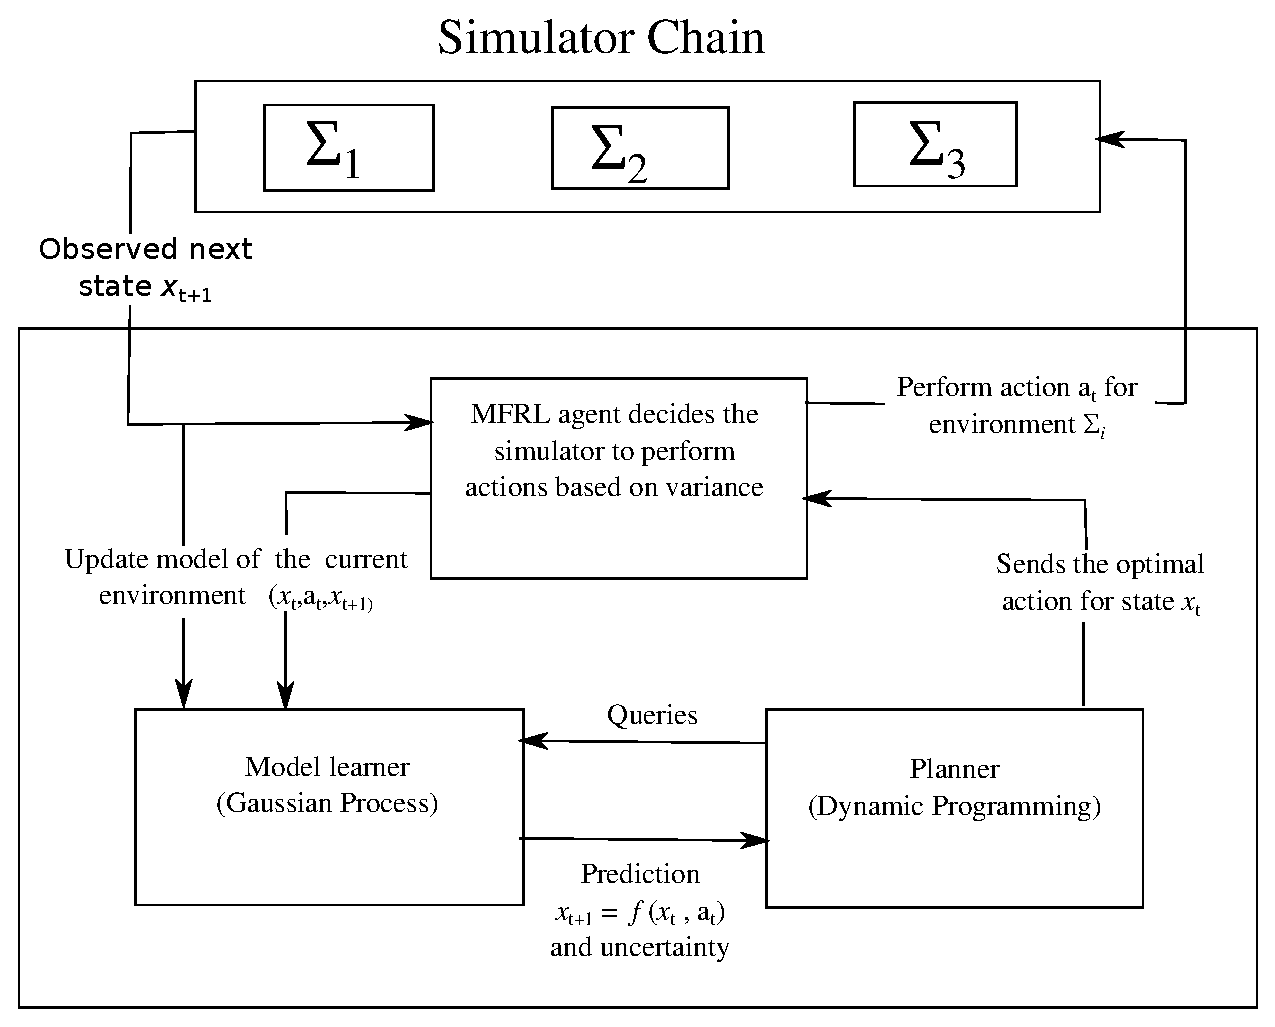
\includegraphics[width=1\columnwidth]{gp-mfrl.eps}
	\caption {Overview of the GP-MFRL algorithm }
   \label{fig:gp_mfrl_system}
\end{figure}

We observe a number of transitions: $\mathcal{D} = \{(\textbf{x}_t, a_t, \textbf{x}_{t+1})\}$. Let $\textbf{x}_{t+1} = f(\textbf{x}_t, a_t)$ be the (unknown) transition function that must be learned. Our goal is to learn an estimate $\tilde{f}(\textbf{x}, a)$ of $f(\textbf{x}, a)$ in as few samples in $\mathcal{D}$ as possible. We can then use this estimated $\tilde{f}$ for unvisited state-action pairs (in place of $f$) during value iteration to learn the optimal policy. $f$ can also be a stochastic transition function, in which case, the GP estimate gives the mean and the variance of this noisy transition function. For a given state-action pair $(s,a)$, the estimated transition function is defined by a normal distribution with mean and variance given by:
\begin{equation}\label{gaussian_mean}
\mu_{(s,a)|\mathcal{D}} = \mathcal{K}_{(s,a)\mathcal{D}}\mathcal{K}^{-1}_{\mathcal{D}\mathcal{D}}\vec{\mathcal{X}}_{\mathcal{D}} 
\end{equation}
\begin{equation}\label{gaussian_variance}
\sigma^2_{(s,a)|\mathcal{D}} = \mathcal{K}\{(s,a),(s,a)\}-\mathcal{K}_{(s,a)\mathcal{D}}\mathcal{K}^{-1}_{\mathcal{D}\mathcal{D}}\mathcal{K}_{(s,a)\mathcal{D}}
\end{equation}
where $\mathcal{K}$ is the kernel function.

GP regression requires a kernel which encodes the correlation between the values of $f$ at two points in the state-action space. Choosing a right kernel is the most crucial step in implementing GP regression. We choose the Radial Basis Function (RBF) kernel for our implementation since it models the spatial correlation we expect to see in an aerial robot system well. However, any appropriate kernel can be used in our algorithm depending on the environment to be modeled. 

RBF has infinite dimensional feature space and satisfies the Lipschitz smoothness assumption. It can be defined as follows: for two points $\textbf{x}$ and $\textbf{x'}$,
\begin{equation} \label{kernel_def}
\begin{split}
k(\textbf{x}, \textbf{x'})= \exp\bigg(-\frac{|| \textbf{x}-\textbf{x'}||^2}{2\sigma^2}\bigg)\end{split}
\end{equation}
where $||\textbf{x}-\textbf{x'}||^{2}$ is the squared Euclidean distance and $\sigma$ is a hyperparameter for the kernel often known as \textit{characteristic length-scale}. Here, $\textbf{x}$ represents a point in the joint state-action space.

Instead of using GPs to predict the next state, we use it to predict the velocity with which the robot will move when a given action $a_t$ is applied at a state $s_t$. Learning the velocity vector helps in transitioning between simulators as the size of the state space itself may be different. For example, one can construct a multi-fidelity simulator where $\Sigma_0$ is a $n\times n$ grid, $\Sigma_1$ is a denser $2n\times 2n$ grid, and so on. An action in $\Sigma_0$ moves the robot one unit whereas the same action in $\Sigma_1$ moves the robot only 0.5 units. By learning the velocity instead of the next state, we can scale the learned velocity function to easily compute the transition function in any $\Sigma_i$ as:
\begin{equation} \label{velocity_def}
\begin{split}
\vec{\mathcal{V}} \ (s_t,a_t) = \frac{s_{t+1}-s_t}{\Delta_i} 
\end{split}
\end{equation}
where $\Delta_i$ is the time scaling of a simulator. If the state spaces of all simulators are the same, then one can use GPs to predict the next state instead of the velocity vector.

We train two GP regressions, $f_x,f_y:\mathbb{R}^4\rightarrow\mathbb{R}$, assuming independence between the two output dimensions. Let $(x_i,y_i)$ be the current state of the agent. Actions actions are represented using a tuple $(a_x,a_y)$ where $a_x$ and $a_y$ can take the values between $0$ or $1$. 

The GP prediction is used to determine the transitions, $(x_i,y_i,a_x)$ $\rightarrow$ $x_{i+1}$ and $(x_i,y_i,a_y)$ $\rightarrow$ $y_{i+1}$ where $(x_{i+1},y_{i+1})$ is the predicted next state with variance $\sigma_x$ and $\sigma_y$ respectively. Value of hyperparameters is estimated by gradient descent by optimizing the maximum likelihood estimate of a training data set. 


\section{GP-MFRL Algorithm}

Using multiple approximations of real world environments has previously been considered in the literature~\cite{abbeel2006using,taylor2007transfer}. Cutler et al. used model-based R-Max algorithm to reduce the number of samples using MFRL framework \cite{cutler2014reinforcement}. We use GP regression to further bring down the empirical sample complexity of MFRL framework. 


Algorithm~\ref{GP-MFRL} gives the details of the proposed framework. As illustrated in Figure~\ref{fig:gp_mfrl_system}, there are two main components of GP-MFRL: (1) Model Learner; and (2) Planner. The model learner in our case is the GP-regression described in the previous subsection. We use value iteration~\cite{sutton1998reinforcement} as our planner to calculate the optimal policy on learned dynamics of environment. 

An \emph{epoch} measures the time span between two consecutive switches in the simulators. Before executing an action, the agent checks (Step 4) if it has a sufficiently accurate estimate of the transition dynamics for the current state-action pair in the lower fidelity simulator, $\Sigma_{d-1}$. If not, it switches to $\Sigma_{d-1}$ and executes the action in the potentially less expensive environment. The function $\rho^{-1}$ checks if the current state is also a valid state in the lower fidelity simulator. 

We also keep track of the variance of the $\mathcal{L}$ most recently visited state-action pairs in the current epoch. If the running sum of the variances is below a threshold (Step 8), this suggest that the robot has found a good policy in the current simulator and it must advance to the next higher fidelity simulator.

Steps 12--16 in describe the main body where the agent computes the optimal action, executes it, and records the observed transition in $\mathcal{D}$. The GP model is updated after every $n_U$ iterations (Step 17). In the update, we recompute the hyper-parameters until they converge.

A new policy is computed every time the robot reaches the goal state (Step 21). If the robot is in the highest fidelity simulator, we also check if the policy has converged by checking if the maximum change in the value function is less than a threshold (Step 22). If so, we terminate the learner.
\pagebreak

\addtolength{\topmargin}{-.875in}

\begin{algorithm}

\SetKwData{Left}{left}\SetKwData{This}{this}\SetKwData{Up}{up}
\SetKwFunction{Learner}{Learner}\SetKwFunction{Planner}{Planner}\SetKwFunction{UpdateGP}{UpdateGP}\SetKwFunction{epochLength}{epochLength}
\SetKwInOut{Input}{Input}\SetKwInOut{Output}{Initialize}
\Input{A simulator chain,\\ Confidence parameter $\psi$ for $(s,a)$,\\ History Length $\mathcal{L}$, \\ Confidence $\Psi$, \\ State mapping $\rho$, \\ Reward dynamics $\mathcal{R}_{ss'}^a$ \\ Update rate $n_U$ }
\Output{Transition dynamics $\mathcal{P}_{ss'}^a$ ; \\ $d = 1$ ;\\ $\mathcal{V}^{*}_d(s) \leftarrow $  \Planner ($\mathcal{P}_{ss'}^a$)}
%\BlankLine
%\KwData {text}
%\emph{special treatment of the first line}\;
\SetKwProg{myalg}{}{}{}
\myalg{\Learner{}}{
\While{\textnormal{true} }{
\emph{$a^{*}_t \leftarrow \underset{}{\textnormal{argmax}_a}$ $\mathcal{V}^{*}_d(s_t)$} \;
\If(\tcp*[h]{Return to level $d - 1$}){$\sigma(\rho^{-1}(s_t,a^{*}_t) \geq \psi \ \bigwedge \ d > 1 $}{\label{lt}
%\lIf{\Left $<$ \This}{\Union{\Left,\This}}
%\lElse{\Union{\This,\Left}}
\emph{$d \leftarrow d-1$}\;
\epochLength $\leftarrow \ 0$
}
%\tcp*[h]{Path length covered $\leftarrow$ 0}
\If{$\sum_{i = t - \mathcal{L}}^{t-1}\sigma(s_i, a_i^{*}) \leq \Psi \  \bigwedge  \epochLength \geq \mathcal{L}$}{\label{forins}
$d \leftarrow d + 	1$ \ (Move up the simulator) \;
\epochLength $\leftarrow \ 0$ \; }

$a^{*}_t \leftarrow {\textnormal{argmax}_a}$ $\mathcal{V}^{*}_d(s_t)$\;
\emph{\textnormal{Execute}  $a^{*}_t $ \textnormal{and store observed} $s_{t+1}, r_{t+1}$ \;
\epochLength $++$ \;
$\mathcal{D}_t=\mathcal{D}_t \cup (s_{t}, \ a^{*}_t  , \ s_{t+1})$}\; 
$s_{t} \leftarrow s_{t+1}$ \;
\If{\epochLength \textnormal{is multiple of $n_U$}  }{\label{forins1}
\emph{$\mathcal{P}^a_{ss'} \leftarrow \UpdateGP(\mathcal{D}_t) $}\;}

\If{ $s_t$ \textnormal{is Goal state}}{\label{forins2}
\emph{$\mathcal{V}_f(s) \leftarrow \Planner(\mathcal{P}_{ss'}^a)$} \;

\If{ \textnormal{${\textnormal{max}_s} \ \mathcal{V}_f (s) - \mathcal{V}_0 (s) \leq 10 \ \% \bigwedge d == D$}}{\label{forins3}
break the loop \;
}
$\mathcal{V}_0 (s) \leftarrow \mathcal{V}_f $\;
}

$t \leftarrow t + 	1$ \;


%}

%\lForEach{element $e$ of the line $i$}{\FindCompress{p}}
}}
\SetKwProg{myproc}{}{}{}
\myproc{\Planner{}}{
%\Input{Reward dynamics $\mathcal{R}_{ss'}^a$ }
\Output{$\mathcal{V}(s)=0, \ \forall (s,a)$ \\ $\Delta = \infty$}
\While{$\Delta > 0.1$}{\label{forins4}
\For{every s:}{
\emph{$temp \leftarrow \mathcal{V}(s) $} \;
\emph{$\mathcal{V}(s) \leftarrow   \textnormal{max}_a \sum_{a} \sum_{s'} \mathcal{P}_{ss'}^a[\mathcal{R}_{ss'}^a+\gamma  \mathcal{V}(s')] $}\;
\emph{$\Delta \leftarrow \textnormal{max}(0, \  |temp - \mathcal{V}(s)|)$}
}
}
\emph{return $\mathcal{Q}(s,a)$}
}
\caption{GP-MFRL Algorithm}\label{GP-MFRL}
\end{algorithm}



\section{Simulation Results} \label{gp-mfrl-sim}
We demonstrate the GP-MFRL algorithm in a simulator chain consisting of a virtual gridworld environment and the Gazebo robot simulator~\cite{koenig2004design}. The setup is shown in Figure \ref{fig:gp_mfrl_setup}. The simple grid-world agent operates in a $21\times 21$ grid. The agent receives a reward of $+50$ at the goal location, and $-1$ for all other states. If the agent hits the obstacles, it gets the reward of $-20$. In each time step, an agent can move in one of the four directions viz. up, down, left and right. We add a Gaussian noise of $\sigma$ to the actual transition to represent stochastic environments. The Gazebo simulation setup consists of a quadrotor with PX4 autopilot running in software--in--the--loop (SITL) mode. The PX4 SITL interfaces with the Robot Operating System~\cite{quigley2009ros} via the \texttt{mavros} node. 

The code is written in python and uses scikit-learn \cite{scikit-learn} to implement GP-regression. The code is available online at \url{https://github.com/raaslab/gp_gazebo}.

\begin{figure}[htp]
	\centering
	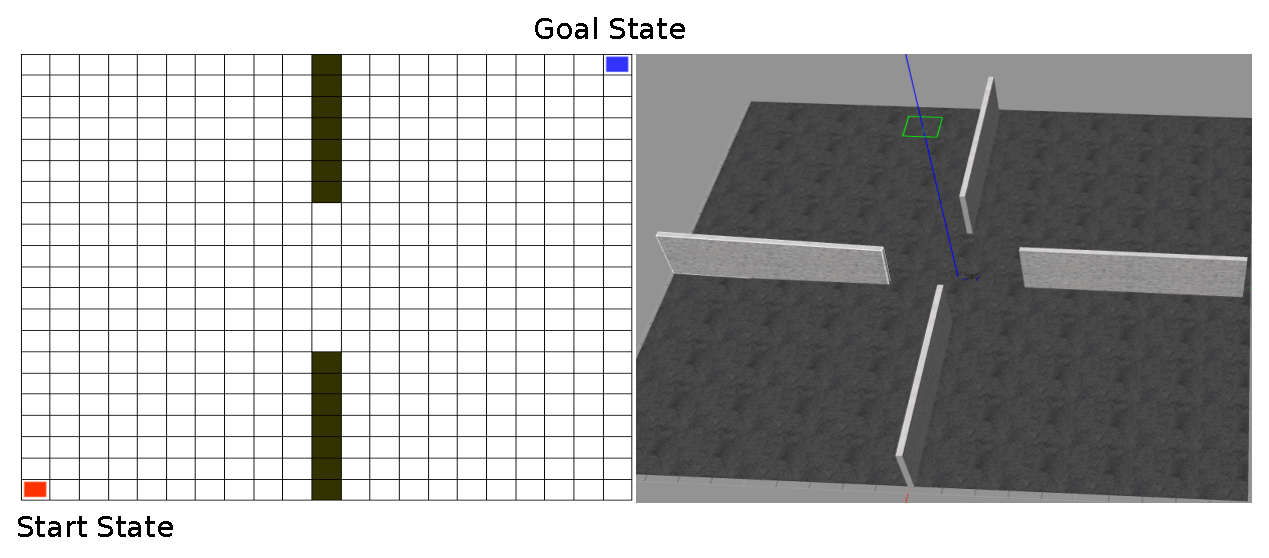
\includegraphics[width=1\columnwidth]{env.eps}
	\caption{The environment setup for a multi-fidelity simulator chain. The simple gridworld environment has two wall obstacles whereas the gazebo environment has four wall obstacles as shown.}
   \label{fig:gp_mfrl_setup}
\end{figure}

Figure~\ref{fig:epoch_samples} shows the switching between the simulators for one run of the GP-MFRL algorithm on the environment shown in Figure~\ref{fig:gp_mfrl_setup}. It can be seen that the agent switches back and forth between the two simulators unlike unidirectional transfer learning algorithms. In the rest of the simulations we study the effect of the parameters used in GP-MFRL and the fidelity of the simulators on the number of samples till convergence.
\begin{figure}[htp]
	\centering 
    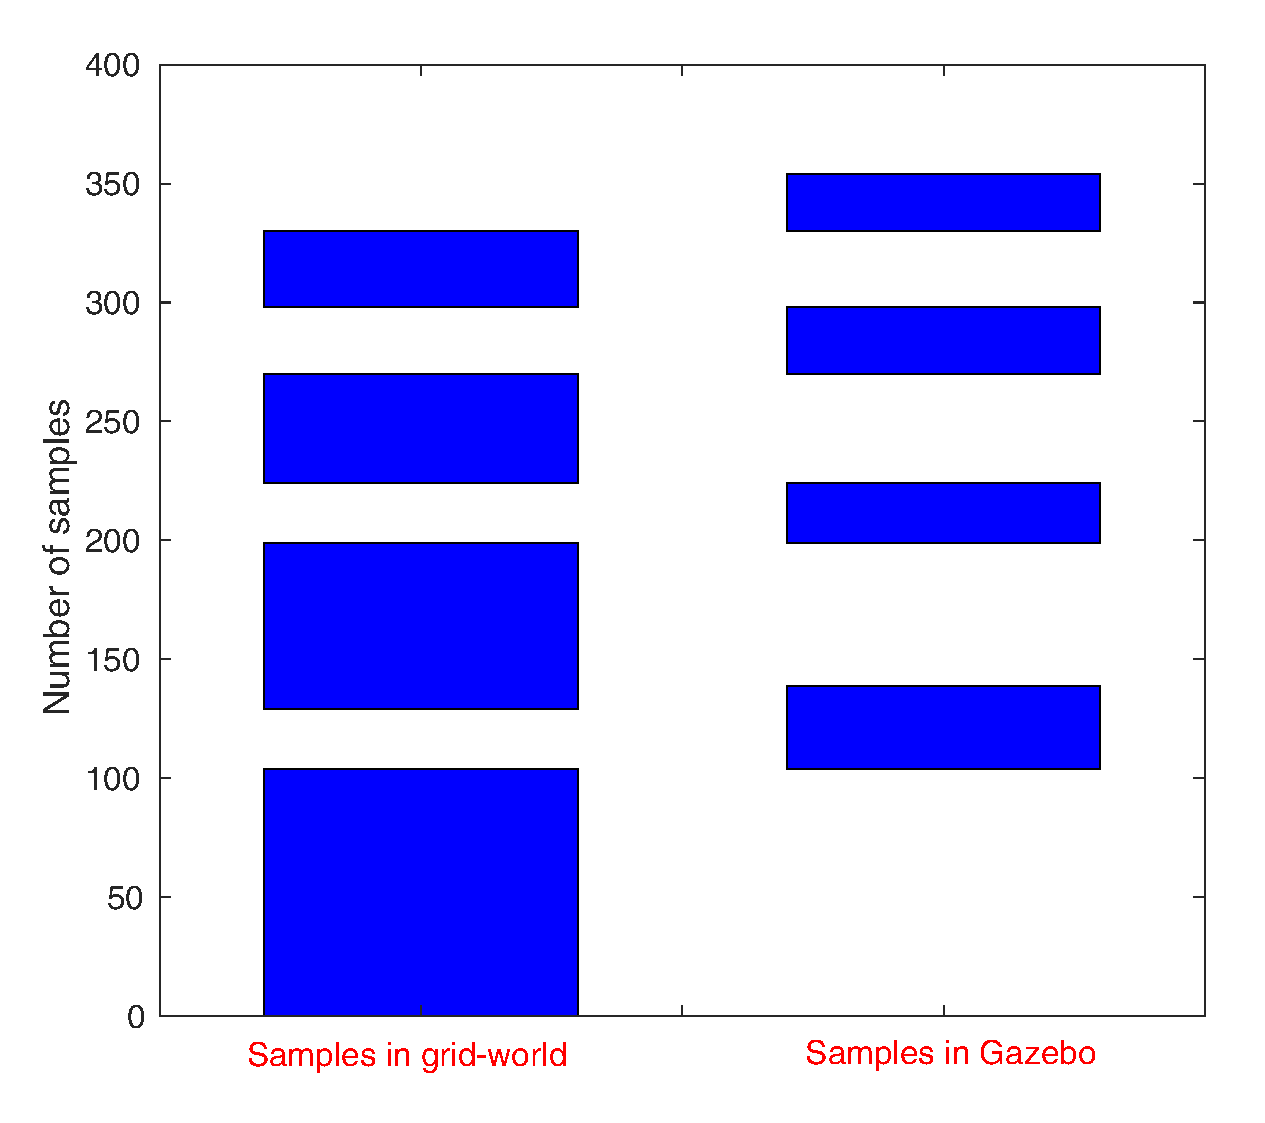
\includegraphics[width=6cm]{epoch.eps}
	\caption{ The figure represents the samples collected in each level of simulator for a $21 \times 21$ grid in a simple grid-world and Gazebo environments. $\Psi$ and $\psi$ were kept 0.4 and $0.1$}
   \label{fig:epoch_samples}
\end{figure}

\subsection{Representative simulations}
We first present three representative scenarios to observe the qualitative performance of the GP-MFRL algorithm. Specifically, we consider three instances and show how the variance evolves over time as more samples are collected. Recall that the main advantage with using GPs is that it allows for quick generalization of observed samples to unobserved state-action pairs.

To demonstrate how variance of the predicted transition dynamics varies from the beginning of experiment to convergence, we plot ``heatmaps'' of the variance. The GP prediction for a state-action pair also gives the variance, $\sigma_x$ and $\sigma_y$, respectively for the predicted state. The heatmap shows $\sqrt{\sigma_x^2 + \sigma_y^2}$ for the optimal action at every state as returned by the Planner. 

Figures~\ref{fig:heatmap1} and \ref{fig:heatmap2} show the heatmaps at the start and convergence for the same environment but with different start and goal positions. As expected, the variance along the optimal (\ie, likely) path is low whereas the variance for states unlike to be on the optimal path from start to goal remains high. 

\begin{figure}
	\centering
    \subfigure[After Initial Training]{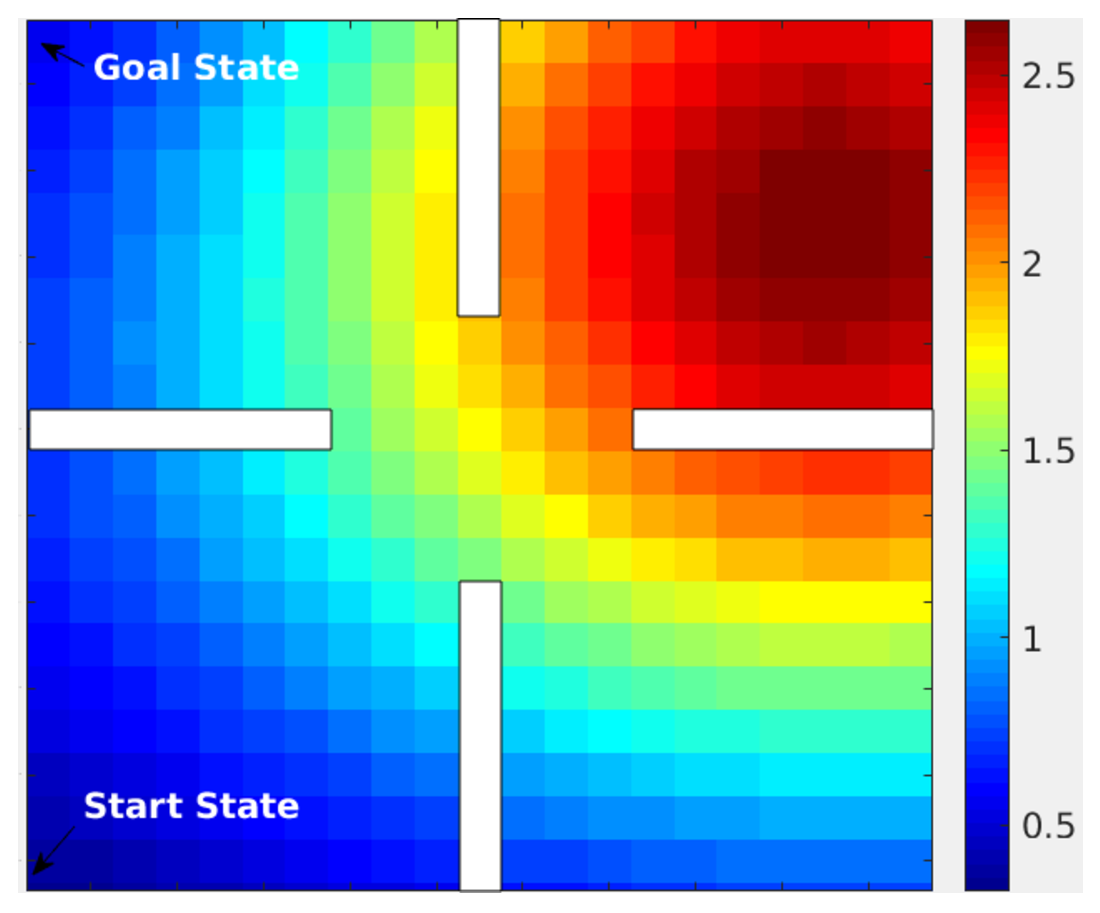
\includegraphics[width=4cm]{heat_init_same.eps}}
    \subfigure[After Convergence]{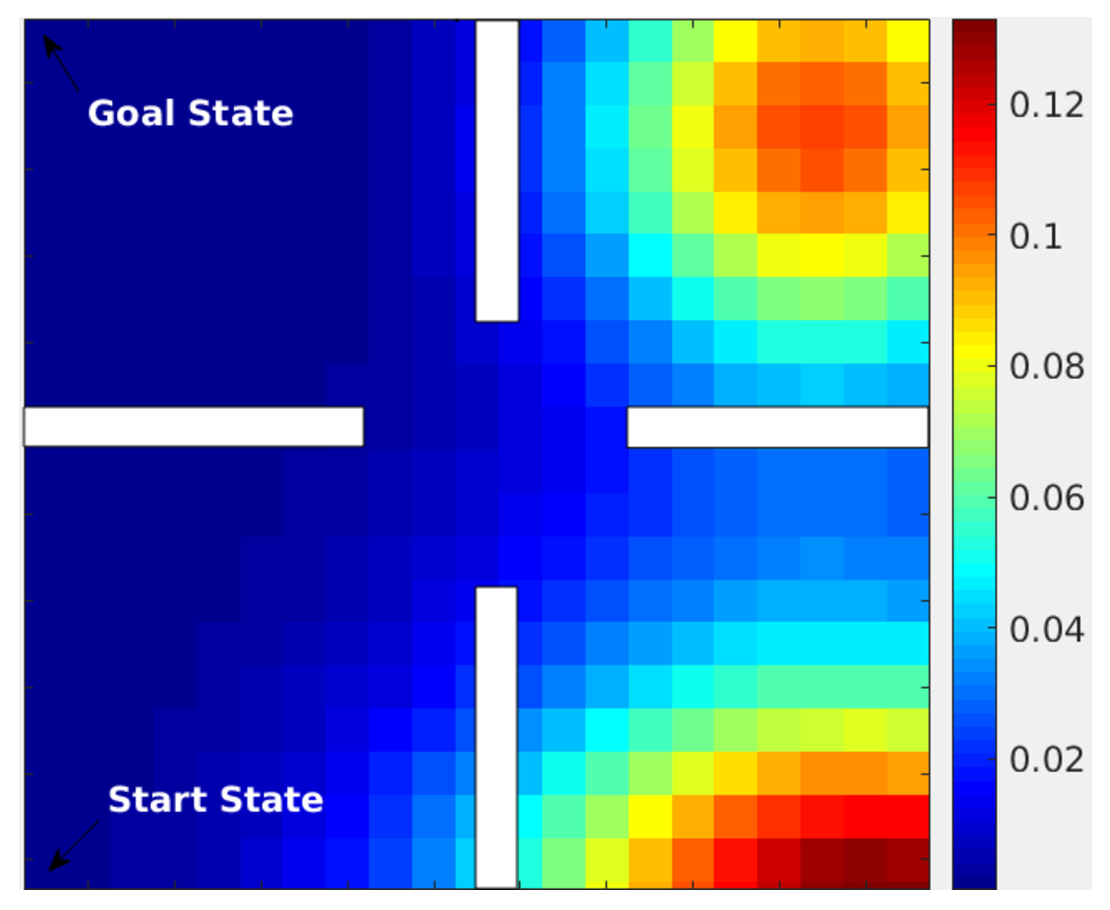
\includegraphics[width=4cm]{heat_same.eps}}
	\caption{Variance plot for $21 \times 21$ multi-fidelity environment after transition dynamics initialization and after algorithm has converged}
   \label{fig:heatmap1}
\end{figure}

\begin{figure}[htp]
	\centering 
    \subfigure[After Initial Training]{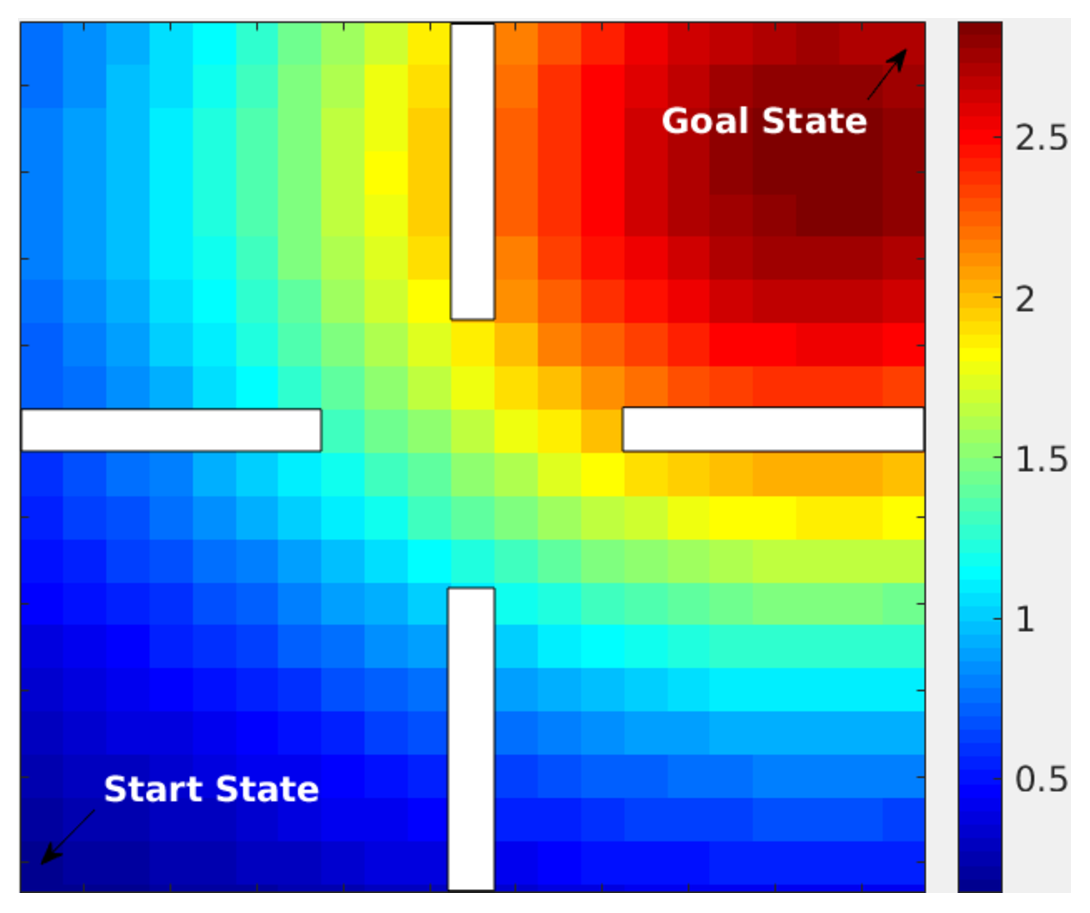
\includegraphics[width=4cm]{heat_init_opposite.eps}}
    \subfigure[After Convergence]{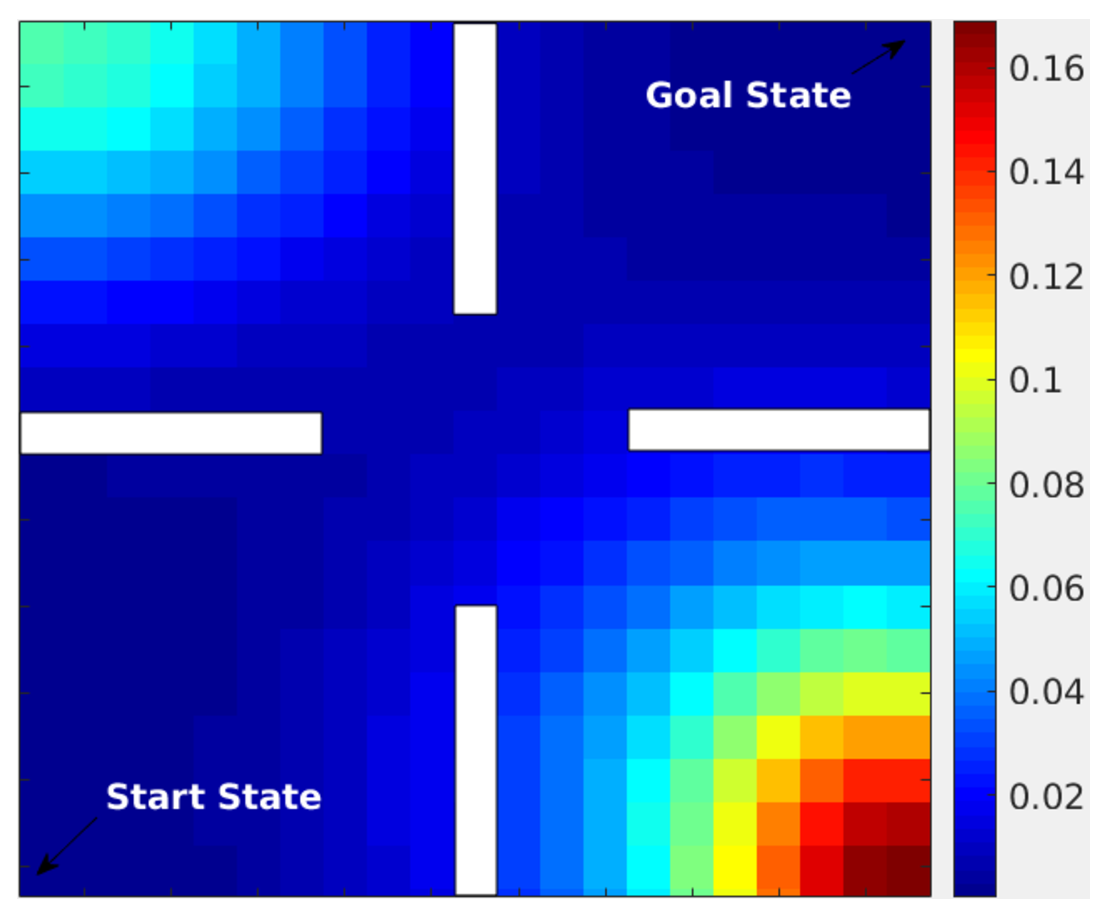
\includegraphics[width=4cm]{heat_opposite.eps}}
	\caption{Variance plot for $21 \times 21$ multi-fidelity environment after transition dynamics initialization and after algorithm has converged}
   \label{fig:heatmap2}
\end{figure}

A more interesting case is presented in Figure \ref{fig:heatmap_four_walls_complex}. Even though there's a path available to reach the goal from the right of wall A, the agent explores that region less than the region near the walls B, C and D (indicated in dark blue showing less variance). This is due to the fact that, the transition dynamics learned in the lower fidelity simulator is used in the higher fidelity simulator leading to lesser exploration of the regions which are not along the optimal path.
\begin{figure}[htp]
	\centering 
	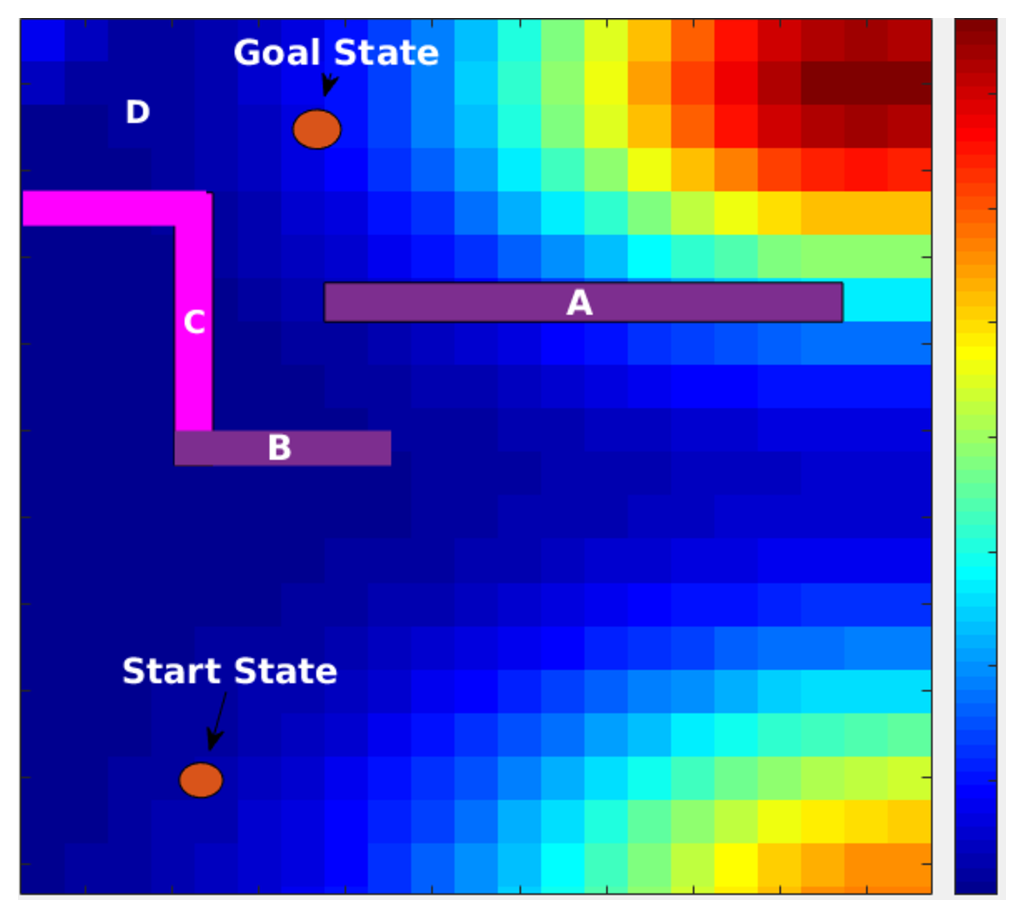
\includegraphics[width=6cm]{heatmap_new.eps}
	\caption{Variance plot for $21 \times 21$ multi-fidelity environment after the algorithm has converged. Walls A and B are only present in the grid-world simulator, whereas all four walls are present in the Gazebo simulator.}
   \label{fig:heatmap_four_walls_complex}
\end{figure}


\subsection{Effect of fidelity on the number of samples.}

We first study the effect of varying fidelity on the total number of samples and the fraction of the samples collected in the higher fidelity simulator. Our hypothesis is that having learned the transition dynamics in the gridworld, the agent will need fewer samples in the higher fidelity Gazebo simulator to find the optimal policy. However, as the fidelity of the first simulator decreases, we would need more samples in Gazebo. 

In order to validate this hypothesis, we varied the noise parameter used to simulate the transitions in the gridworld. The transition model in Gazebo remains the same. The total number of samples collected increases as we increase the noise in gridworld (Figure \ref{fig:gp_mfrl_samples}). As we increase the noise in the first simulator, the agent learns less accurate transition dynamics leading to collection of more number of samples in the higher fidelity simulator. Not only does the agent need more samples, the ratio of the samples collected in the higher fidelity simulator to the total number of samples also increases (Figure \ref{fig:gp_mfrl_ratio}). 


\begin{figure}[htp]
	\centering
	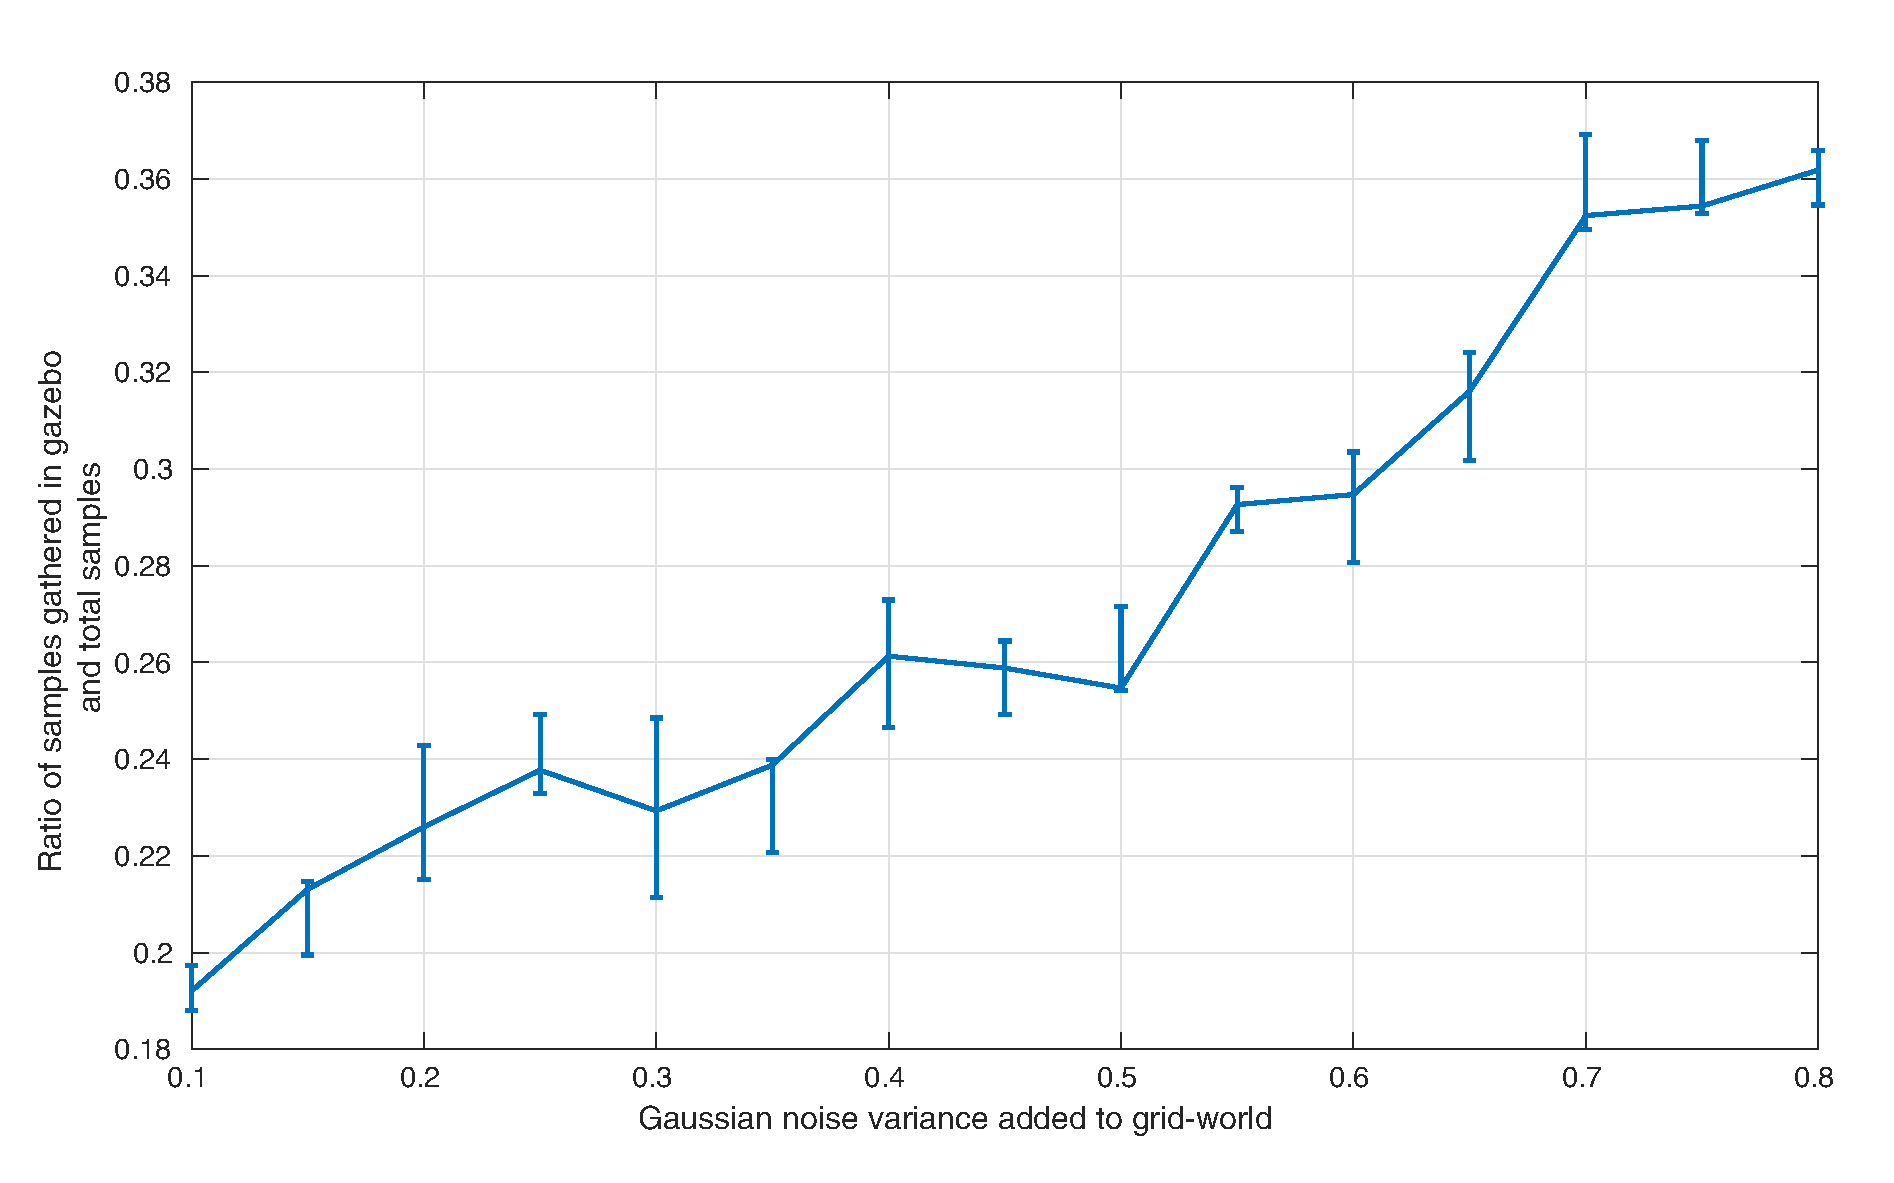
\includegraphics[width=8cm]{ratio.eps}
	\caption{As we make first simulator more inaccurate by adding noise, the agent tends to gather more samples in second simulator }
   \label{fig:gp_mfrl_samples}
\end{figure}

\begin{figure}[htp]
	\centering
	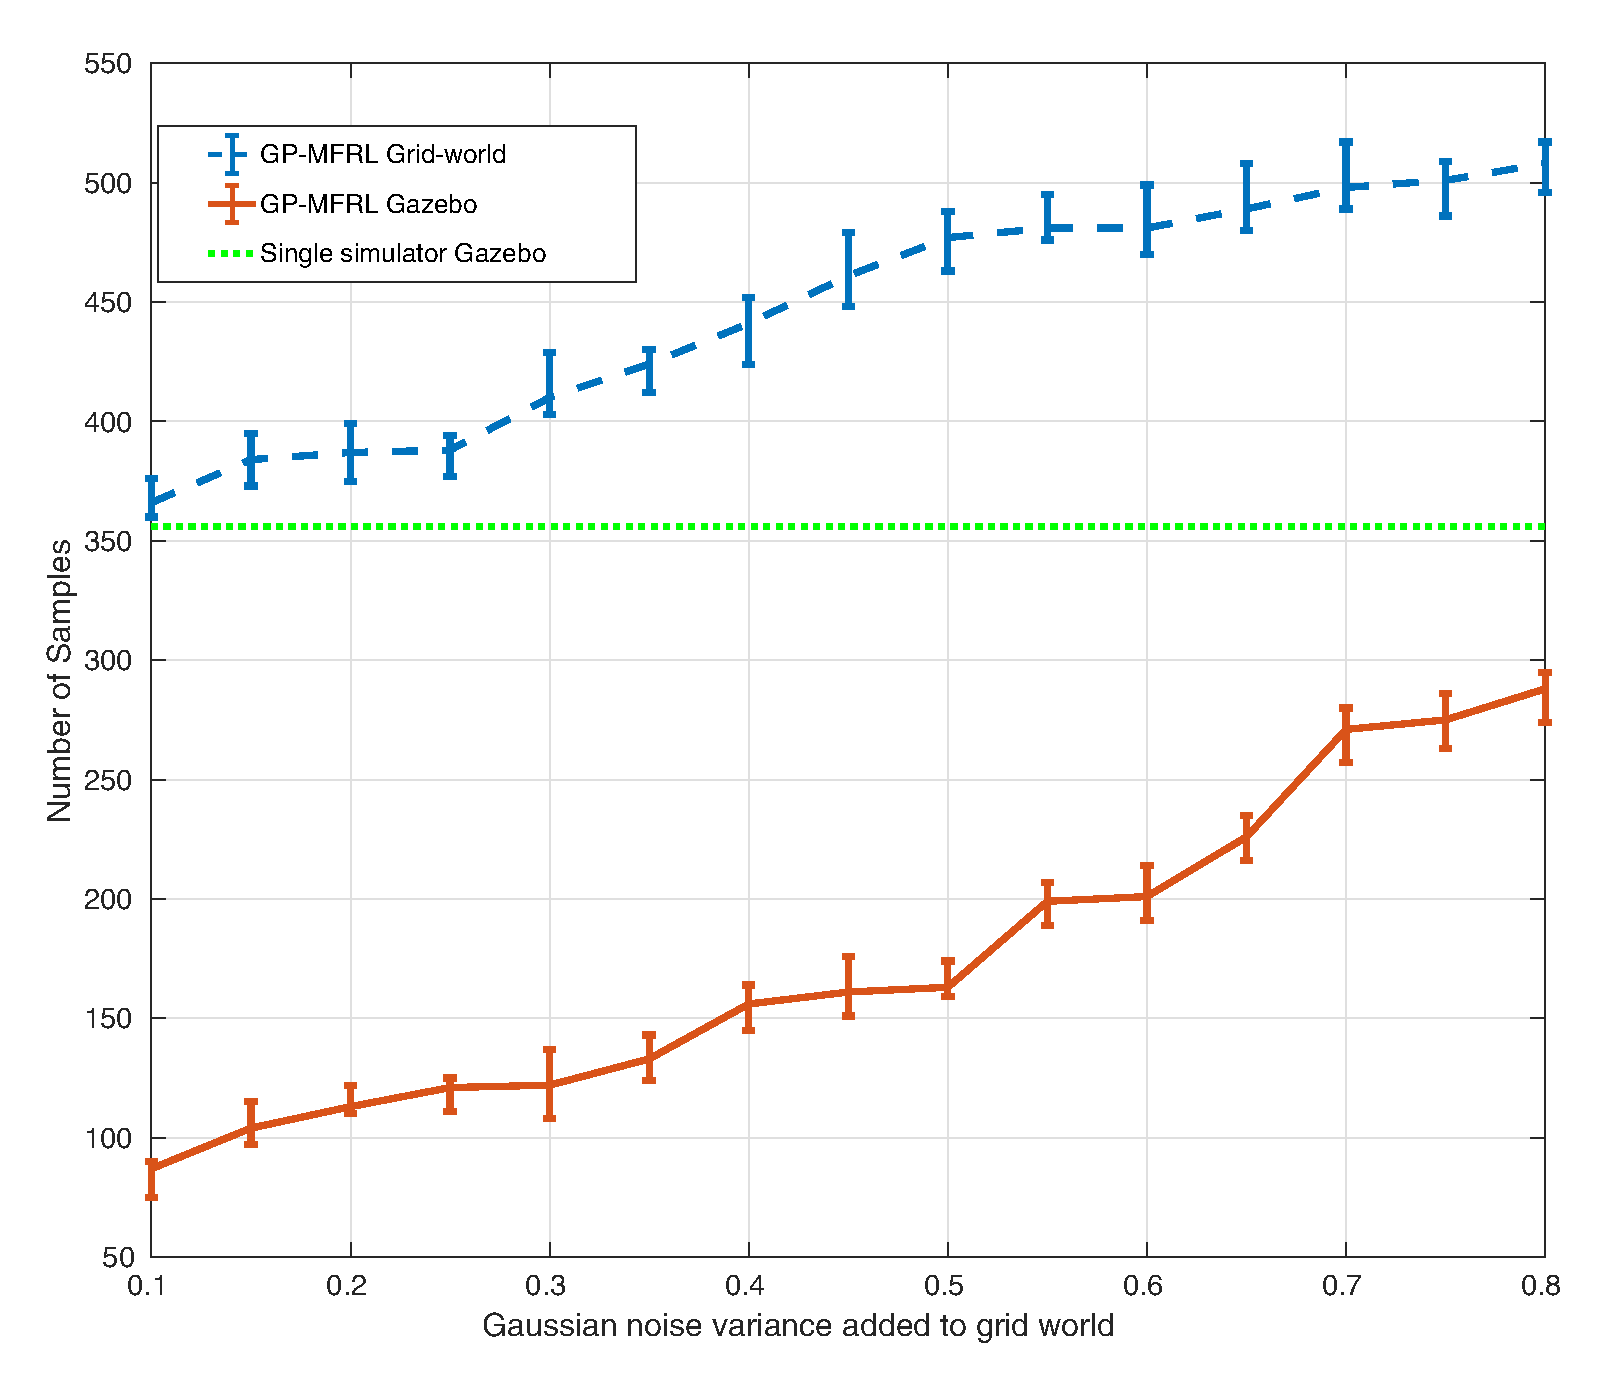
\includegraphics[width=8cm]{samples_gathered_.eps}
	\caption{Ratio of samples gathered in the second simulator to the total samples gathered increases with inaccuracy in the first simulator. The reference line depicts the average number of samples gathered over $10$ runs when only Gazebo simulator was present.}
   \label{fig:gp_mfrl_ratio}
\end{figure}

\subsection{Effect of the confidence parameters.}
The GP-MFRL algorithm uses two confidence parameters, $\psi$ and $\Psi$, which are compared against the variance in the transition dynamics to switch to a lower and higher simulator, respectively. Figure~\ref{fig:threshold} shows the effect of varying the two parameters on the ratio of number of samples gathered in the Gazebo simulator to the total number of samples. As expected, increasing $\psi$ or decreasing $\Psi$ leads to more samples being collected in the higher fidelity simulator. 

\begin{figure}[htp]
	\centering
	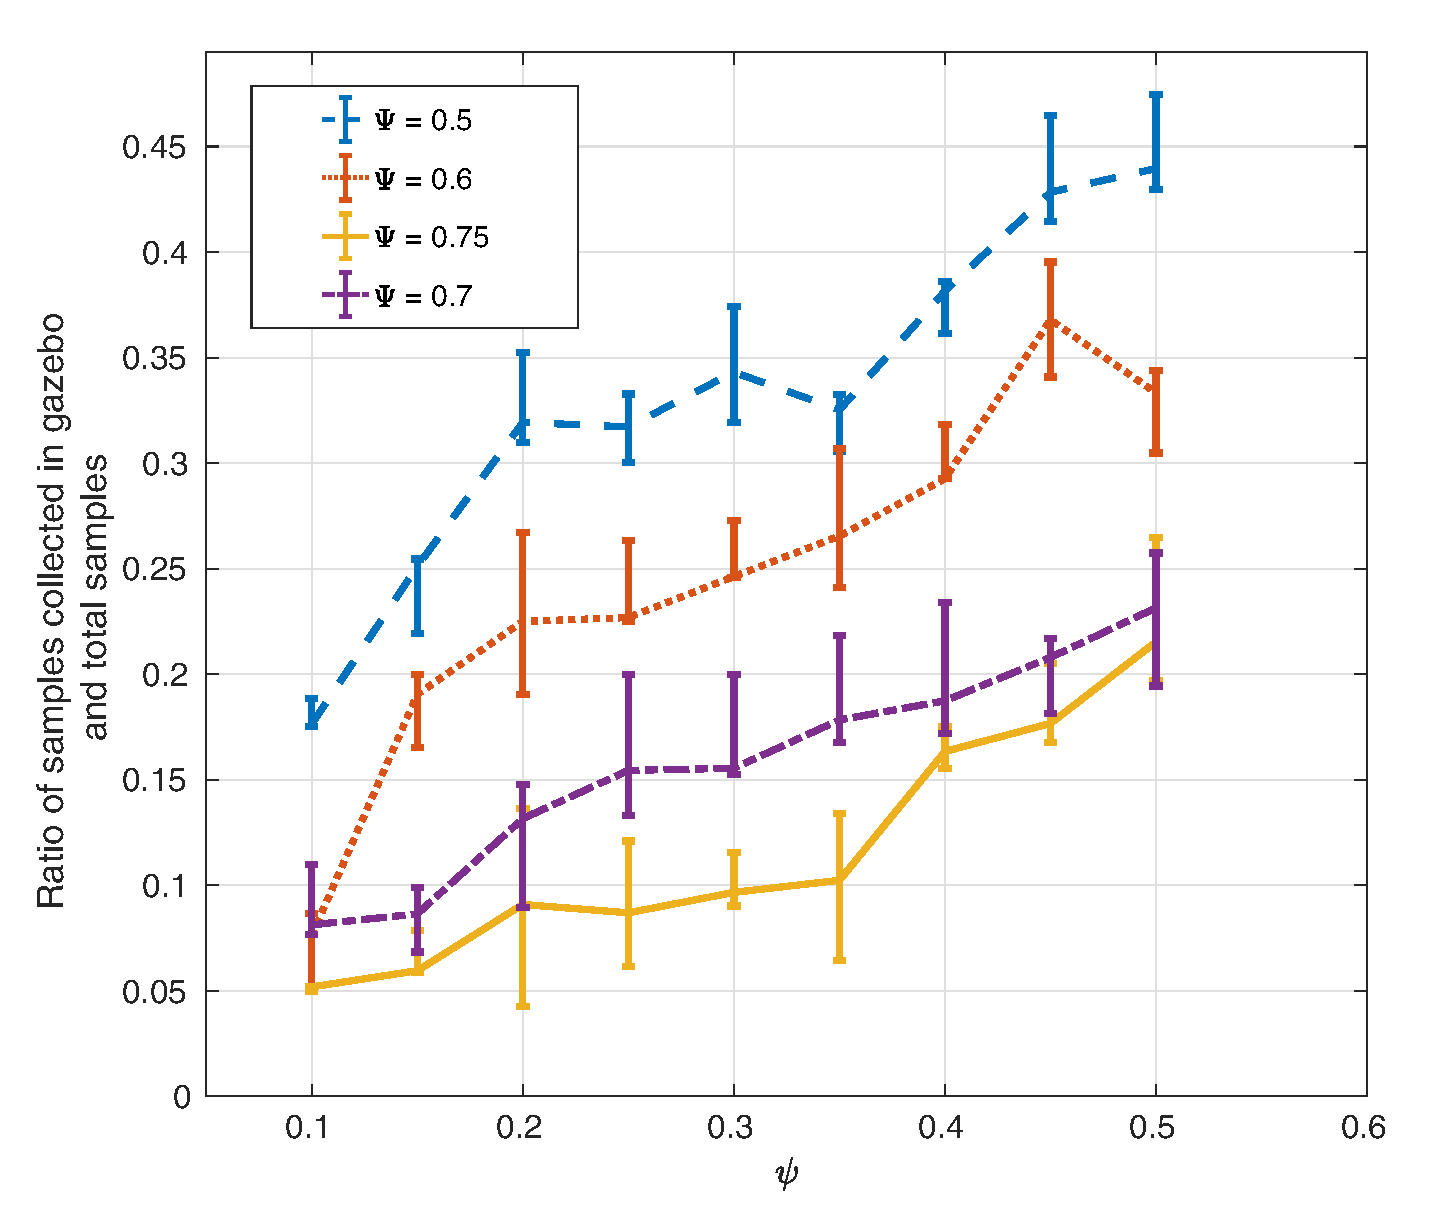
\includegraphics[width=8cm]{thre.eps} 
	\caption{Ratio of samples gathered in second simulator vs. total samples gathered as we change the threshold or confidence parameters of the two simulators.}
   \label{fig:threshold}
\end{figure}

\subsection{Comparison with R-max MFRL}
Figure \ref{fig:value_function} shows the comparison between performance of GP-MFRL algorithm with the existing MFRL algorithm \cite{cutler2014reinforcement}, GP-MFRL algorithm only in the highest fidelity simulator and Rmax algorithm running only in the highest fidelity simulator. The experiments are performed in the environment same as the one used in Figure \ref{fig:heatmap_four_walls_complex}. As expected, the GP-MFRL algorithm performs better than the existing MFRL algorithm, \cite{cutler2014reinforcement}.
\begin{figure}[htp]
	\centering 
    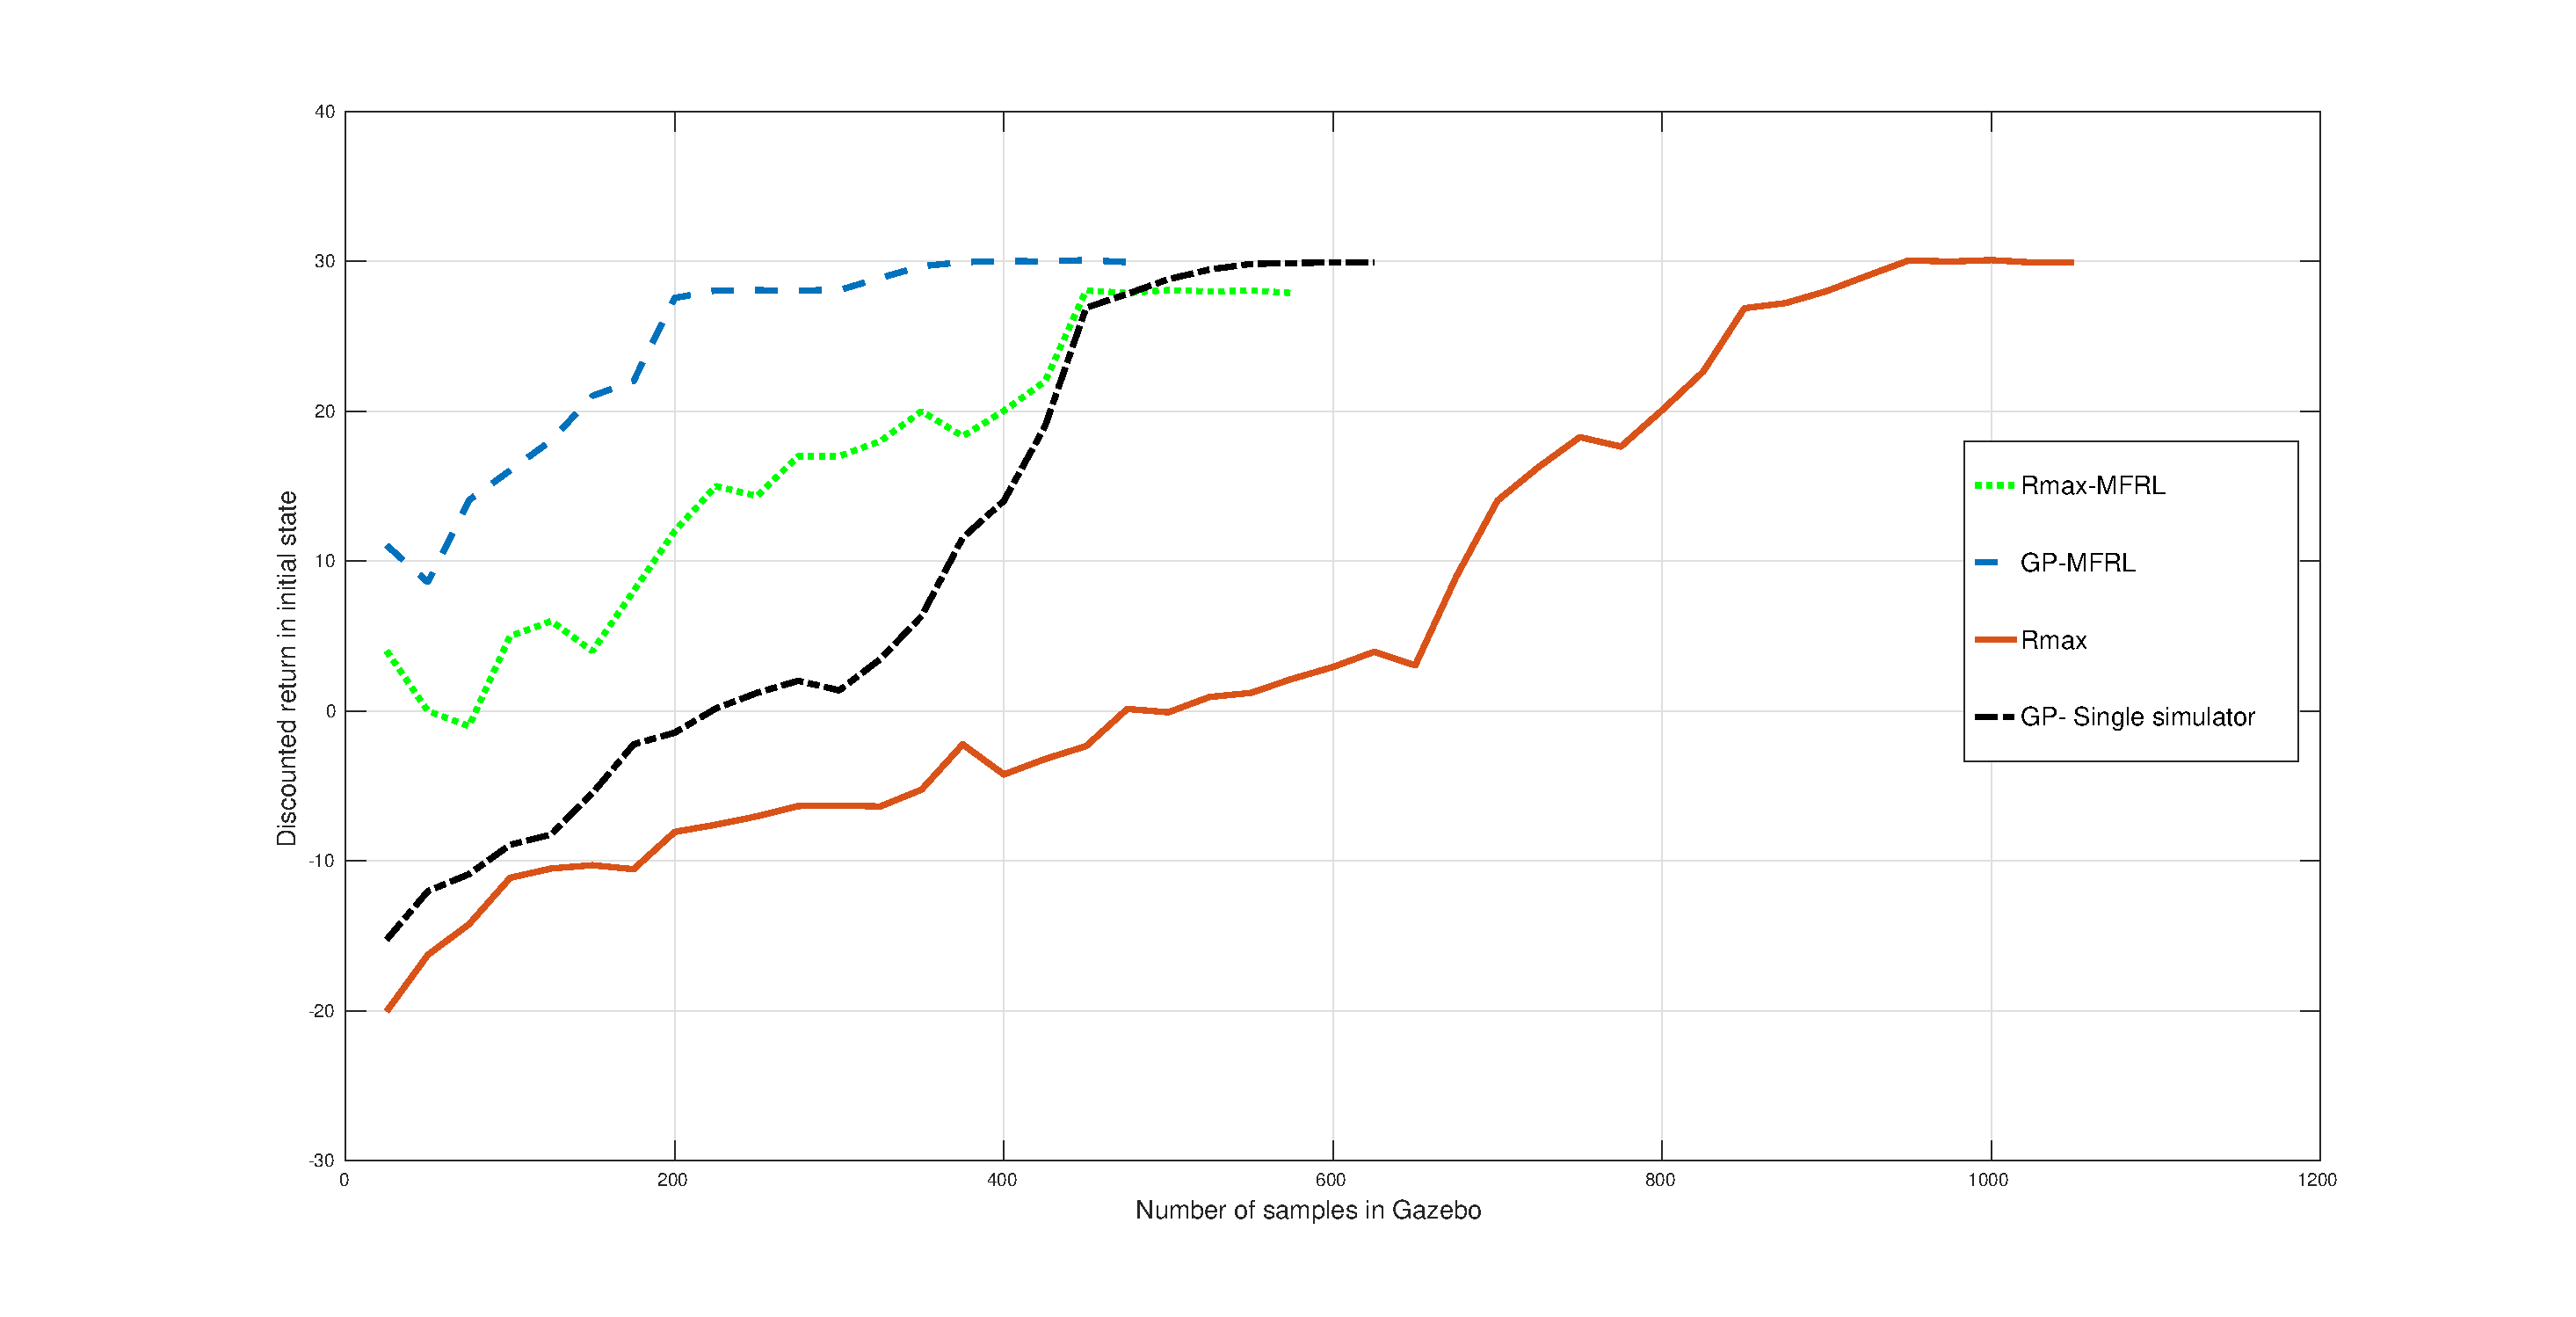
\includegraphics[width=8cm]{reward.eps}
	\caption{ Discounted return in the start state Vs. the number of samples collected in the highest fidelity simulator.}
   \label{fig:value_function}
\end{figure}

\section{Conclusion}
The GP-MFRL algorithm provides a general RL technique that is particularly suited for robotics. An extension to the existing work would be implementing the GP-MFRL algorithm on an actual quadrotor as the highest-fidelity simulator to demonstrate the utility of GP-MFRL. In this thesis, it is shown empirically that, GP-MFRL finds optimal policies using fewer samples than MFRL algorithm. 


\chapter{Bridge Inspection}

%%%%%%%%%%%%%%%%%
%
% Include an EPS figure with this command:
%   \epsffile{filename.eps}
%

%%%%%%%%%%%%%%%%
%
% Do tables like this:
\begin{comment}
 \begin{table}
 \caption{The Graduate School wants captions above the tables.}
\begin{center}
 \begin{tabular}{ccc}
 x & 1 & 2 \\ \hline
 1 & 1 & 2 \\
 2 & 2 & 4 \\ \hline
 \end{tabular}
\end{center}
 \end{table}
\end{comment}
%%%%%%%%%%%%%%%%%%%%%%%%%%%%%%%%

% If you are using BibTeX, uncomment the following:
\bibliography{refs}
\bibliographystyle{plain}
%
% Otherwise, uncomment the following:
% \chapter*{Bibliography}

% \appendix

% In LaTeX, each appendix is a "chapter"
% \chapter{Program Source}


\end{document}